\Chapter{Ütközésvizsgálat}
\label{Chap:utkozesvizsgalat}

% TODO: Ütközéssel, metszéspontokkal kapcsolatos számítások

%- A try bullet-es példa részletes kifejtése, matematikai része

%Egyszerűbb változatoktól a bonyolultabbak fel

%- Először az intuitív, egyszerűbb megoldások, még ha kevésbé hatékony is.
%- Felsorolni több megoldást is.
%- Optimalizálási módszerek részletezése
%- Összehasonlítani őket pontosság és számításigény szempontjából.

Ebben a fejezetben az ütközésvizsgálattal kapcsolatos számításokról, optimalizációkról lesz szó. Ütközésvizsgálatra több szempontból is szükség van. Egyrészt, vizsgálni kell, hogy a játékos a játszható területen belül van-e, azaz nem mehet át falakon, tereptárgyakon, nem mehet fel túl meredek emelkedőn. Másrészt, vizsgálni kell, hogy a játékos által leadott lövedék eltalálja-e a domborzatot, tereptárgyakat, jelezni kell a lövedék becsapódását. Harmadrészt regisztrálni kell az ellenfeleket eltaláló leadott lövéseket. A második és harmadik pont nagyon hasonló, de még is szétszedtem, mert az ellenfeleknél nem a látható geometriát találjuk el, hanem annak egy leegyszerűsített modelljét, a számítások felgyorsítása érdekében. Szükség van további optimalizációkra is, mert ha ezek nem lennének, irreálisan nagy erőforrás igénye lenne a játékoknak.

\section{A karakterek ütközésvizsgálata mozgás szempontjából}

Ez a játék szempontjából az egyik legfontosabb elem. Az hogy kirajzoltatunk valamit a képernyőre, még nem jelenti azt, hogy azon nem lehet áthaladni. A kirajzolás csak a vizualitást adja, a domborzat, a tereptárgyak, a karakterek kinézetét. A játékfejlesztő feladata az, hogy megírja külön az ezekhez szükséges ütközésvizsgálatot. Mivel ez két különálló dolog, egyes helyzetekben adódhatnak olyan problémák, hogy ezek nincsenek szinkronban, tehát látunk valamit amin át lehet menni, vagy nem látunk valamit és mégis megakadunk benne.

Ebben a játékban a karakterek ütközésvizsgálata gradiens számítással van megoldva. Ez azt jelenti, hogy ha két, egymás mellett lévő pont magasságértéke között túl nagy a különbség pozitív irányba, az falat, vagy túl meredek emelkedőt jelent. Ha mérsékelt, vagy nagyon minimális a különbség, akkor arról vagy lecsúszik, vagy csak egyszerűen át lehet ott haladni. Mindezt a beolvasott magasságmezőből számolja, ezzel dinamikussá téve az ütközésvizsgálatot. Ha ez nem lenne így, akkor elveszne a játék azon tulajdonsága, hogy dinamikusan lehet cserélgetni a pályákat minden további nélkül.

Ezen felül a gravitáció ami nagyon lényeges, mert a pályának vannak olyan magaslati pontjai, amelyekre fel lehet jutni. Ha egy ilyenre felmegyünk, és nincs semmilyen erő, ami a karaktert a föld felé húzná, akkor felfelé ugyan lekövetné a talajmagasságot, de le már nem esne alacsonyabb pontra onnan.

 Ez esetben egy lefelé ható erő folyamatosan hat a játékosra és ellenfelekre, aminek a küszöbértéke mindig az aktuális talajmagasság. Ennek pszeudokódja:

\begin{verbatim}
1. gravitációs erő := -9,8;
2. küszöbérték := aktuális talajmagasság;
3. ha karakter függőleges pozíciója > küszöbérték
4. 	akkor
5.		függőleges gyorsaság = függőleges gyorsaság + gravitációs erő;
6.		karakter függőleges pozíciója = karakter függőleges pozíciója 
										+ függőleges gyorsaság;
6.	különben
7. 		karakter függőleges pozíciója = küszöbérték;
\end{verbatim}
 
\section{A domborzat és tereptárgyak üközésvizsgálata a lövés szempontjából}

Az ilyen fajta ütközésvizsgálat számítás nem létszükséglet a játszhatóság szempontjából, de tény, hogy jóval realisztikusabbá teszi a játékot, és sok optimalizációt igényel. Ez teszi lehetővé, hogy ha lövünk egyet, és beletalál bármilyen elembe, ami a pálya része, megjeleníthessük rajta a találatot. Ennek minősége lehet többféle, csak egy textúra, vagy egyéb még realisztikusabb megoldások.

\begin{figure}[h]
\centering
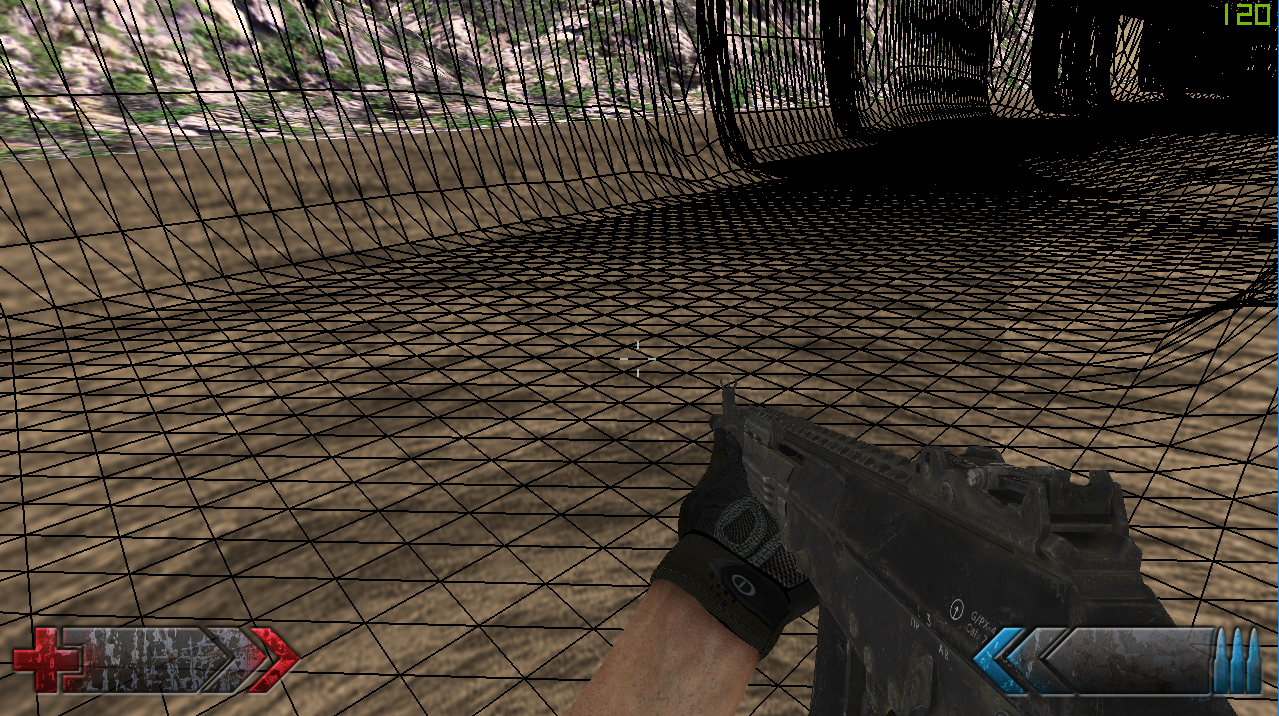
\includegraphics[scale=0.4]{kepek/map_wireframe.png}
\caption{A térkép geometriájának határvonalai}
\label{fig:wireframe}
\end{figure}



\section{A játékos, és az ellenfelek hitboxa}

f


